% Intended LaTeX compiler: pdflatex
\documentclass[10pt,a4paper,UTF8]{article}
\usepackage{zclorg}
\usepackage{tikztheorem}
\author{emacsun}
\date{}
\title{生成模型(generative model)}
\hypersetup{
 pdfauthor={emacsun},
 pdftitle={生成模型(generative model)},
 pdfkeywords={},
 pdfsubject={},
 pdfcreator={Emacs 25.0.50.1 (Org mode 9.0.6)},
 pdflang={English}}
\begin{document}

\maketitle
\tableofcontents
\titlepic{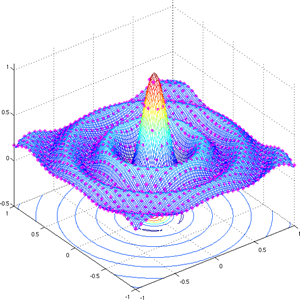
\includegraphics[scale=0.25]{../../img/sinc.PNG}}
我们从判决理论导出生成模型(generative model)是机器学习中经常用到的一种模型。

\section{判决理论}
\label{sec:orgf42d483}


假设我们有一个训练集合(由输入\(\mathbf{x}\)和对应的输出\(\mathbf{t}\)组成),我们的目标是对于给定新的输入\(x\),预测其输出\(t\)。对于回归问题\(t\)是连续的,对于分类问题\(t\)是离散的。如果我们能够得到\(p(x,t)\)的联合分布就好了,因为这个联合分布包含了关于\(x\)这个随机变量的所有不确定度的描述。从一个训练集合中确定\(p(x,t)\)的过程叫做推断(inference)。这个过程难度相当大,尤其当\(x\)的维度非常高时。在实际问题中,我们经常要对\(t\)做预测,或者基于对\(t\)的理解或者预测采取某种动作。这个过程叫做判决(decision)。

以癌症诊断为例,假设我们希望从X光片中预测癌症。输入\(x\)就是X光片,输出\(t\)代表是否有癌症。显然这是一个分类问题。我们用\(\mathcal{C}_{1}\)代表有癌,用\(\mathcal{C}_{2}\)代表无癌。我们也可以用\(t=0\)代表有癌,用\(t=1\)代表无癌。推断问题涉及到\(p(x,t)\)的确定,\(p(x,t)\)告诉我们关于是否致癌的所有信息,我们希望根据\(p(x,t)\)来给出尽可能准确的诊断信息,或者根据\(p(x,t)\)来执行损失最小的行为。

使用贝叶斯准则,给定一个新的X光片时,我们需要知道这个病人是否得癌的概率:
\begin{equation}
\label{eq:1}
p(\mathcal{C}_{k}|x) = \frac{p(x| \mathcal{C}_{k} ) p( \mathcal{C}_{k} )}{p(x)}
\end{equation}
注意上式中的任何量都可以从\(p(x, \mathcal{C}_{k} )\)中导出。\(p( \mathcal{C}_{k} )\)代表\(\mathcal{C}_{k}\)的先验概率,\(p( \mathcal{C}_{k} | x )\)代表后验概率。如果我们的目标是最小化判错概率,那么我们需要较高后验概率的\(\mathcal{C}_{k}\)判为结果。这种判决需要把输入划分成某几个区域\(\mathcal{R}_{k}\),正确的做法是所有位于\(\mathcal{R}_{k}\)的判给\(\mathcal{C}_{k}\)。因此出错的概率为:
\begin{eqnarray}
\label{eq:2}
p(error)&=& p(x\in \mathcal{R}_{1}, \mathcal{C}_{2}) + p(x\in \mathcal{R}_{2}, \mathcal{C}_{1}) \\
&=& \int_{ \mathcal{R}_{1} }p(x, \mathcal{C}_{2} ) \mathrm{d}x + \int_{ \mathcal{R}_{2} } p(x, \mathcal{C}_{1} ) \mathrm{d}x
\end{eqnarray}

稍微有点通信原理基础的同学都晓得这一点和AWGN信道下BPSK信道的接收是一样的。其中判决门限的决定也是一门学问,我们这里是尽可能的使判错的概率降低。但是对于实际的场景可没有那么简单,实际生活中往往要设定某一个损失函数(loss function)使得这个损失函数最小。

\section{三种模型}
\label{sec:orgf860091}


在上一节,我们把分类问题分成两个步骤:1. inference。 这个过程中我们使用训练数据学习了\(p(\mathcal{C}_{k}|x)\);2. decision。在这个过程中我们实用后验概率来做出最优的决定。这个解决办法采用的模型叫做生成模型(generative model)  另外的可能的解决方法是把这两步合二为一:直接学习一个把\(x\)映射为\(\mathcal{C}_{k}\)的函数,这个模型叫做差分模型(discriminant model).

实际上我们有三种解决问题的模型,按照复杂度从高到低来讲,是:
\begin{enumerate}
\item 首先解决inference问题找出\(p(x|C_{k})\)条件概率密度,然后找出\(p(C_{k})\),然后使用贝叶斯公式求出\(p(C_{k}|x)\)。这种模型叫做生成模型,之所以这么命名是因为这个模型对于以后的输入都可以产生比较好的输出。
\item 首先解决\(p(C_{k}|x)\),然后使用判决理论将\(x\)赋值为\(C_{k}\)中的一个。这个模型叫做差分模型。
\item 找到一个差分函数\(f(x)\)把\(x\)映射为\(C_{k}\)中的一种。在这个模型中概率没有扮演任何角色。
\end{enumerate}
\end{document}
